
\documentclass[aps, nofootinbib,superscriptaddress, preprintnumbers, longbibliography]{article}

\usepackage{tikz}
\usepackage{jcappub}
\usepackage[utf8]{inputenc}
\usepackage{amsmath,amsfonts,amssymb}
\usepackage{graphicx}
\usepackage[toc,page]{appendix}
\usepackage{cleveref}
\usepackage[loose]{units}
\usepackage{booktabs}
\usepackage{mathtools}
\setcounter{tocdepth}{2}
\usepackage{listings}
\usepackage{xcolor}

\lstset{
  basicstyle=\ttfamily\small,
  keywordstyle=\color{blue},
  commentstyle=\color{gray},
  numbers=left,
  numberstyle=\tiny,
  stepnumber=1,
  numbersep=5pt,
  frame=single,
  breaklines=true,
  columns=fullflexible,
  backgroundcolor=\color{white},
}

\def\la{~\mbox{\raisebox{-.6ex}{$\stackrel{<}{\sim}$}}~}
\def\ga{~\mbox{\raisebox{-.6ex}{$\stackrel{>}{\sim}$}}~}

\makeatletter
\gdef\@fpheader{}
\makeatother

\title{
	\texttt{InflationEasy}:\\ A C++ Lattice Code for Inflation
}

\author[a]{Angelo Caravano}
\affiliation[a]{Institut d'Astrophysique de Paris, UMR 7095 du CNRS et de Sorbonne Universit\'e,\\ 98 bis bd Arago, 75014 Paris, France}
\emailAdd{caravano@iap.fr}

\abstract{
%We present \texttt{InflationEasy}, a C++ code to simulate single-field inflation on a three-dimensional cubic lattice. The code evolves a scalar field in an expanding FLRW universe using finite differences for spatial derivatives and a staggered leapfrog integrator for time evolution. While partially based on the well-known \texttt{LATTICEEASY}, \texttt{InflationEasy} introduces several improvements and features tailored specifically to inflationary dynamics. Notably, it implements a $\delta N$ method to compute the comoving curvature perturbation $\zeta$ directly from the lattice, enabling a wide range of phenomenological applications including predictions relevant for large-scale structure surveys and gravitational wave interferometers.
We introduce \texttt{InflationEasy}, a C++ code for simulating single-field inflation on a three-dimensional lattice in an expanding FLRW universe. The code evolves the scalar field using finite-difference spatial derivatives and a staggered leapfrog integrator for time evolution. While partially based on the well-known \texttt{LATTICEEASY}, it incorporates several improvements specifically designed for inflationary applications. In particular, \texttt{InflationEasy} implements a nonlinear $\delta N$ formalism to compute the curvature perturbation at the end of inflation $\zeta$ directly from the lattice, making it well suited for scenarios with large fluctuations or non-perturbative non-Gaussianities. The code is lightweight, easy to use, and applicable to a broad range of inflationary models, including those relevant for primordial black hole formation, gravitational wave production, and large-scale structure.
}


\begin{document}
	\maketitle
	
	%%%%%%%%%%%%%%%%%%%%%%%%%%%%%%%%%%%
	\section{Introduction}

Lattice simulations have become essential tools in studying the nonlinear dynamics of the early universe, particularly in regimes where perturbation theory breaks down—such as preheating and cosmological phase transitions. Over the past two decades, several public codes have been developed for this purpose, including \texttt{LATTICEEASY}~\cite{latticeeasy}, \texttt{DEFROST}~\cite{Frolov_2008}, \texttt{PSpectRe}~\cite{Easther_2010}, \texttt{HLattice}~\cite{hlattice}, \texttt{PyCOOL}~\cite{Sainio_2012}, \texttt{GFiRe}~\cite{Lozanov_2020}, and \texttt{CosmoLattice}~\cite{figueroa2021cosmolattice}. These codes have been widely used to simulate nonlinear field dynamics after inflation, especially during reheating. However, none are specifically designed to simulate the inflationary phase itself, far from the end of inflation.~\footnote{An exception is \texttt{STOLAS}~\cite{Mizuguchi:2024kbl}, which simulates inflation using the stochastic inflation formalism, which differs substantially from the standard lattice method of solving differential equations on a fixed comoving grid.}

\texttt{InflationEasy} fills this gap. It is a simple, publicly available C++ code that evolves a canonical scalar field on an expanding 3D lattice during inflation. Designed specifically for inflationary dynamics, it offers an accessible platform to simulate a wide range of single-field models. The code is lightweight, modular, and easy to modify—even for users with minimal experience in C++. One of its main distinctive feature is the implementation of a nonlinear $\delta N$ method to compute the comoving curvature perturbation $\zeta$ directly from the lattice, enabling a fully non-perturbative calculation of non-Gaussianity, crucial in many scenarios such as primordial black hole formation.

\texttt{InflationEasy} has already been employed in several studies~\cite{Caravano:2021pgc,Caravano:2022yyv,Caravano:2024tlp,Caravano:2024xsb,Caravano:2024moy, USR2}, where it has been used to explore a variety of inflationary models and benchmark a fully nonlinear calculation of $\zeta$ based on the $\delta N$ formalism. This paper accompanies the public release of the code and serves both as a feature summary and as a user manual. The public version of the code can be downloaded ~\textcolor{red}{[here]}.

The paper is organized as follows. In \cref{sec:eoms}, we present the physical system and its equations of motion. In \cref{sec:implementation}, we describe the numerical implementation, including discretization, time evolution, and output generation. \Cref{sec:instructions} contains user instructions, including a walkthrough of the default options and how to configure a new potential. We conclude in \cref{sec:conclusions}.

	%Lattice simulations have become essential tools in studying the nonlinear dynamics of the early universe, particularly in regimes where perturbation theory breaks down, such as during preheating or cosmological phase transitions. Several public codes have been developed over the past two decades, including \texttt{LATTICEEASY}~\cite{latticeeasy}, \texttt{DEFROST}~\cite{Frolov_2008}, \texttt{PSpectRe}~\cite{Easther_2010}, \texttt{HLattice}~\cite{hlattice}, \texttt{PyCOOL}~\cite{Sainio_2012}, \texttt{GFiRe}~\cite{Lozanov_2020}, and \texttt{CosmoLattice}~\cite{figueroa2021cosmolattice}. However, none of these are designed to simulate the inflationary phase itself, far from the end of inflation.\footnote{An exception is \texttt{STOLAS}~\cite{Mizuguchi:2024kbl}, which is tailored for inflation but within the stochastic inflation formalism, which differs from the standard lattice approach of solving differential equations on a grid of fixed comoving size.}

%\texttt{InflationEasy} fills this gap by providing a simple yet powerful C++ code that evolves a scalar field on an expanding 3D lattice. Designed specifically for inflation, it is straightforward to operate and to modify the inflationary potential—even for users with no prior experience in C++. The code has been developed and tested in several works~\cite{Caravano:2021pgc,Caravano:2021bfn,Caravano:2022epk,Caravano:2022yyv,Caravano:2024tlp,Caravano:2024xsb,Caravano:2024moy}. This paper accompanies the public release of the code, available at [link]. While the core techniques of the lattice implementation have been described in the associated publications, this document serves both as a summary of the features of the code and as a user manual for the public release.

%This paper is structured as follows. In \cref{sec:eoms}, we review the physical system and equations of motion. In \cref{sec:implementation}, we describe the numerical implementation, including the description of the different outputs and the structure of the code. Sec \ref{sec:instructions} contains user instructions, including a description of the default options and the steps needed to implement a new inflationary potential. \Cref{sec:configuring} explains how to implement a custom inflationary potential. We conclude in \cref{sec:conclusions}.

	%%%%%%%%%%%%%%%%%%%%%%%%%%%%%%%%%%%
	\section{Equations of motion in continuous space}
	\label{sec:eoms}
	%%%%%%%%%%%%%%%%%%%%%%%%%%%%%%%%%%%
	The code solves the Klein-Gordon equation for a canonical scalar field $\phi$ in a flat FLRW spacetime using comoving time:
\begin{equation}
\label{eq:fullcont}
\partial_\tau^2\phi + 2\mathcal{H}\partial_\tau \phi - \nabla^2\phi + a^2\frac{\partial V}{\partial \phi} = 0,
\end{equation}
where $a(\tau)$ is the scale factor and $\mathcal{H} = \partial_\tau a / a$ is the conformal Hubble parameter. A key feature of the lattice approach is that no background/perturbation split is introduced—the inflaton field and its fluctuations are evolved altogether.
The evolution of the scale factor is governed by the Friedmann equations:
\begin{align}
\label{eq:friedmann}
&\mathcal{H}^2 = \frac{1}{3} \langle \rho \rangle a^2,\\
&\frac{d^2a}{d\tau^2} = \frac{1}{6} \left(\langle \rho \rangle - 3 \langle p \rangle\right) a^3,
\end{align}
where $\langle \rho \rangle$ and $\langle p \rangle$ are the average energy density and pressure:
\begin{equation}
\begin{split}
\rho = -T^0_{\hspace{1mm}0} = \frac{(\partial_\tau\phi)^2}{2a^2} + \frac{|\vec\nabla\phi|^2}{2a^2} + V(\phi),\\
p = \frac{1}{3} \sum_i T^i_{\hspace{1mm}i} = \frac{(\partial_\tau\phi)^2}{2a^2} - \frac{|\vec\nabla\phi|^2}{6a^2} - V(\phi).
\end{split}
\label{eq:ED}
\end{equation}
In the code, the gradient term is evaluated via the identity
\[
|\vec\nabla\phi|^2 \equiv -\phi \nabla^2\phi,
\]
which follows from integrating by parts in the action. This trick, inherited from \texttt{LATTICEEASY}, allows reuse of the Laplacian operator used in \cref{eq:fullcont} for evolving the scale factor as well.

To evolve $a(\tau)$ numerically, one of the Friedmann equations must be used. We arbitrarily choose the second equation for time evolution, using the first as an energy conservation check—as done in \texttt{LATTICEEASY}.

 
	\subsection{Neglecting metric perturbations}
	Throughout the simulation, the background spacetime is modeled by the FLRW metric $g_{\mu\nu} = a^2(\tau)(-d\tau^2 + d\vec{x}^2)$, and metric perturbations $\delta g_{\mu\nu}$ are neglected. Setting $\delta g_{ij} = 0$ is a gauge choice—we work in the spatially flat gauge. However, the non-dynamical components $\delta g_{0\mu}$ are in principle constrained by the Einstein equations. These are typically suppressed in slow-roll inflation, where the first slow-roll parameter $\epsilon = -\dot{H}/H^2 \ll 1$ (with $H$ the Hubble parameter and a dot, e.g., $\dot{H}$, denoting derivative with respect to cosmic time $t$). In this regime, neglecting $\delta g_{0\mu}$ is a valid approximation \cite{Caravano:2022yyv,Caravano:2024moy}. This has been recently confirmed by numerical relativity simulations~\cite{Launay:2025kef} which agree well with lattice results using a fixed metric~\cite{Caravano:2022yyv,Caravano:2024tlp,Caravano:2024xsb,Caravano:2024moy}.

When $\epsilon \sim 1$, this assumption breaks down, and one needs to be careful about the role of metric perturbations. Even when $\epsilon \ll 1$, metric perturbations can lead to small but potentially important corrections to observables. In such cases, they can be reintroduced perturbatively as corrections to the effective inflaton mass, as done in~\cite{Caravano:2024xsb}. However, this first public release of \texttt{InflationEasy} does not include these corrections.
	
	
	%%%%%%%%%%%%%%%%%%%%%%%%%%%%%%%%%%%
    \section{Numerical implementation}
    \label{sec:implementation}
    In this section, we provide an overview of the numerical implementation, from the discretization of the equations of motion to the calculation of physical outputs. The content summarized here draws from the developments in~\cite{Caravano:2021pgc,Caravano:2021bfn,Caravano:2022epk,Caravano:2022yyv,Caravano:2024tlp,Caravano:2024xsb,Caravano:2024moy}, and serves as a general introduction to the tools included in the public release of the code. For additional technical details, we refer the reader to these references.

\subsection{Discretization and lattice equations of motion}
\label{sec:discrete}

To solve \cref{eq:fullcont} numerically, we discretize space on a cubic lattice. The lattice consists of $N_{\rm pts}^3$ points, separated by a comoving lattice spacing $\Delta x = L / N_{\rm pts}$, where $L$ is the comoving physical length of the simulation box. A continuous field $f(\vec{x})$ is mapped to a discrete array $f(\vec{n})$:
\begin{equation}
\label{eq:discretization}
f(\vec{x}), \quad \vec{x} \in \mathbb{R}^3 \quad\longrightarrow\quad f(\vec{n}), \quad \vec{n} \in \mathbb{N}^3,\quad n_i \in \{1, \dots, N_{\rm pts}\}.
\end{equation}
We impose periodic boundary conditions so that, for example, $f(N_{\rm pts}, n_2, n_3) = f(1, n_2, n_3)$. Under this discretization, the partial differential equation \cref{eq:fullcont} becomes a system of $N_{\rm pts}^3$ coupled ordinary differential equations:
\begin{equation}
\label{eq:disc}
\partial_\tau^2 \phi(\vec{n}) + 2\mathcal{H}\partial_\tau \phi(\vec{n}) - [\nabla^2 \phi](\vec{n}) + a^2 \frac{\partial V}{\partial \phi}(\vec{n}) = 0.
\end{equation}
The coupling arises through the discrete Laplacian $[\nabla^2 \phi](\vec{n})$, which we define using a second-order central finite-difference stencil~\cite{press1986numerical}:
\begin{equation}
\label{eq:discretelaplacian}
[\nabla^2 f](\vec{n}) = \frac{1}{(\Delta x)^2} \sum_{\alpha = \pm 1} \left(
f(\vec{n} + \alpha \vec{e}_1) + f(\vec{n} + \alpha \vec{e}_2) + f(\vec{n} + \alpha \vec{e}_3) - 3f(\vec{n})
\right),
\end{equation}
where $\vec{e}_1 = (1, 0, 0)$, $\vec{e}_2 = (0, 1, 0)$, and $\vec{e}_3 = (0, 0, 1)$. This approximation converges to the continuum Laplacian as $\Delta x \rightarrow 0$, with a truncation error of order $O(\Delta x^2)$. While higher-order stencils can be implemented for greater accuracy (as discussed in Appendix C of~\cite{Caravano:2021pgc}), the present public release includes only the second-order scheme.

\subsubsection{Modified dispersion relation}
\label{sec:modified}

Discretizing space alters the dynamics of waves on the lattice compared to continuous space. To see this, consider the wave equation for a free scalar mode:
\begin{equation}
\partial_\tau^2 \psi(\vec{x}, \tau) = \nabla^2 \psi(\vec{x}, \tau) \quad \xrightarrow{\text{FT}} \quad \partial_\tau^2 \psi(\vec{k}, \tau) = -k^2 \psi(\vec{k}, \tau),
\end{equation}
where FT denotes a Fourier transform. In discrete space, the finite-difference Laplacian yields a different evolution in Fourier space:
\begin{equation}
\partial_\tau^2 \psi(\vec{n}, \tau) = [\nabla^2 \psi](\vec{n}, \tau) \quad \xrightarrow{\text{DFT}} \quad \partial_\tau^2 \psi(\vec{\kappa}, \tau) = -k_{\rm eff}^2(\vec{\kappa}) \psi(\vec{\kappa}, \tau),
\end{equation}
where $\vec{\kappa}$ is the discrete lattice momentum,
\begin{equation}
\vec{\kappa} = \frac{2\pi}{L} \vec{m}, \quad \vec{m} \in \mathbb{N}^3, \quad m_i \in \{1, \dots, N_{\rm pts}\},
\end{equation}
and the effective wavenumber $k_{\rm eff}$ is given by
\begin{equation}
\label{eq:eff}
\vec{k}_{\rm eff}(\vec{\kappa}) = \frac{2N_{\rm pts}}{L} \sin\left( \frac{\pi \vec{m}}{N_{\rm pts}} \right).
\end{equation}
This defines a modified dispersion relation that converges to the continuum form $k^2$ only in the infrared: $k_{\rm eff}(\vec{\kappa}) \to |\vec{\kappa}|$ when $m_i \ll N_{\rm pts}$. Thus, wave propagation on the lattice differs from that in continuous space due to the discreteness of the grid.

This issue can be resolved by identifying $\vec{k}_{\rm eff}(\vec{\kappa})$ with the physical momentum $\vec{k}$ of the corresponding continuum mode:
\begin{equation}
\vec{k}_{\rm eff}(\vec{\kappa}) \longleftrightarrow \vec{k}.
\end{equation}
This observation, introduced in~\cite{Caravano:2021pgc}, implies that the lattice evolution is equivalent to continuum evolution if one interprets momenta using $k_{\rm eff}$. While we illustrated this equivalence for a free wave equation, it has also been shown to hold for inflationary dynamics in single-field models~\cite{Caravano:2021pgc,Caravano:2022yyv}. This is not true in general—for instance, in axion-gauge models such as axion-$U(1)$ inflation, this prescription is insufficient~\cite{Caravano:2021bfn,Caravano:2022epk}, and one must resort to higher-order schemes or spectral differentiation.

In \texttt{InflationEasy}, this effective wavenumber prescription is used to correct for discretization both in setting the initial conditions and in computing output observables such as the inflaton power spectrum. As a result, outputs such as power spectra become insensitive to the choice of lattice spacing, making this one of the key improvements over other lattice codes.

\subsubsection{Equations in code units}

The code works in rescaled spatial and temporal coordinates $(\tilde{x}, \tilde{\tau})$, defined via
\begin{equation}
\label{eq:rescaling}
d\tau \rightarrow d\tilde{\tau} = B a^s\, d\tau, \quad x \rightarrow \tilde{x} = Bx,
\end{equation}
where $B$ is a constant with dimensions of inverse length and $s$ is a dimensionless scaling parameter. This rescaling is inspired by the conventions of \texttt{LATTICEEASY}, and enhances the numerical stability of the equations.

In these rescaled variables, the equations of motion take the form:
\begin{align}
\label{eq:eoms}
\begin{split}
&\partial_{\tilde{\tau}}^2 \phi + (2 + s)\frac{\partial_{\tilde{\tau}} a}{a} \, \partial_{\tilde{\tau}} \phi - a^{-2s} [\tilde{\nabla}^2 \phi] + a^{2 - 2s} \frac{\partial \tilde{V}}{\partial \phi} = 0,\\
&\partial_{\tilde{\tau}}^2 a = -s \frac{(\partial_{\tilde{\tau}} a)^2}{a} + \frac{1}{3} a^{-2s + 3} \left( \langle \tilde{\rho} \rangle - 3 \langle \tilde{p} \rangle \right),
\end{split}
\end{align}
where all quantities with tildes have been normalized by appropriate powers of $B$ (e.g., $\tilde{V} = V / B$). The spatial derivatives $[\tilde{\nabla}^2 \phi]$ are computed using the same finite-difference stencil described earlier, but now expressed in terms of the rescaled lattice spacing $\tilde{\Delta x} = B\Delta x$.

Internally, all evolution is carried out in these code units. However, to improve interpretability, all output quantities of the code (e.g., power spectra, background observables) are automatically converted to reduced Planck units.

	%%%%%%%%%%%%%%%%%%%%%%%%%%%%%%%%%%%
	
\subsection{Initial Conditions}
\label{sec:ic}
%%%%%%%%%%%%%%%%%%%%%%%%%%%%%%%%%%%

We now describe the generation of initial conditions on the lattice. While the procedure follows the standard approach used in most lattice simulations, \texttt{InflationEasy} includes one significant improvement: the initial fluctuations are generated in a way that accounts for the modified dispersion relation induced by the lattice, as discussed in \cref{sec:modified}. This feature, first introduced in~\cite{Caravano:2021pgc}, ensures consistency between the initialization and the discrete dynamics.

Although the evolution of the field is fully non-perturbative—with no background/perturbation split introduced—the initial conditions do rely on such a separation. Specifically, the field is initialized as a classical background plus quantum fluctuations. We now describe the initialization of these two components.

\subsubsection{Background values}

The initial background values of the inflaton $\bar{\phi}(\tilde\tau_{\rm in})$ and its velocity $\partial_{\tilde\tau} \bar{\phi}(\tilde\tau_{\rm in})$ are set according to the homogeneous inflationary trajectory, i.e. the solution to \eqref{eq:fullcont} without the gradient term. The scale factor is initialized as $a = 1$, and its time derivative in program units is determined from the Friedmann equation using the background energy density:
\begin{equation}
\label{eq:initial_H}
3\,\partial_{\tilde\tau} a(\tilde\tau_{\rm in}) = \bar\rho = \frac{(\partial_{\tilde\tau} \bar\phi(\tilde\tau_{\rm in}))^2}{2} + V(\bar\phi).
\end{equation}
After generating the fluctuations (as described below), the initial value of $\partial_{\tilde\tau} a$ is updated to include the contribution from the gradient energy, computed as a lattice average of $(\vec{\tilde\nabla} \phi)^2 / 2$. While quantum vacuum fluctuations should not source the background equations, their inclusion here reflects the semi-classical approximation used in the lattice approach. Importantly, omitting this gradient term would introduce a residual curvature term into the second Friedmann equation, compromising the consistency of the evolution. Including it also enables accurate monitoring of energy conservation during the simulation, as discussed in \cite{latticeeasy,Caravano:2022yyv}.

\subsubsection{Fluctuations}

We now describe the initialization of field fluctuations. A detailed derivation can be found in~\cite{Caravano:2022yyv}, but we summarize the main steps here.

We begin by defining the discrete version of the Bunch-Davies vacuum:
\begin{equation}
\label{eq:discBD}
u(\vec\kappa) = \frac{L^{3/2}}{a \sqrt{2 \omega_{\vec\kappa}}} e^{-i \omega_{\vec\kappa} \tau}, \quad\quad \omega_{\vec\kappa}^2 = k_{\rm eff}^2(\vec\kappa) + m^2 \simeq k_{\rm eff}^2(\vec\kappa),
\end{equation}
where we have neglected the inflaton mass $m$, which is typically small during slow-roll. The normalization factor $L^{3/2}$ accounts for the finite volume of the lattice box (see~\cite{Caravano:2022yyv} for details). Crucially, this mode function incorporates the lattice-corrected dispersion relation via $k_{\rm eff}$, as defined in \cref{eq:eff}, in contrast to standard approaches which use the lattice momenta $\vec{\kappa} = 2\pi \vec{m} / L$.

To generate classical field fluctuations, we assign each Fourier mode a random complex amplitude drawn from a Rayleigh distribution with variance $|u(\vec\kappa)|^2$:
\begin{equation}
\label{eq:randommodes}
\phi(\vec\kappa) = e^{i 2\pi Y_{\vec{\kappa}}} \sqrt{-\ln(X_{\vec{\kappa}})} \, u(\vec\kappa),
\end{equation}
where $X_{\vec{\kappa}}$ and $Y_{\vec{\kappa}}$ are independent random variables uniformly distributed in $(0, 1)$. 

An inverse discrete Fourier transform is then applied to obtain the real-space field configuration. The fluctuations are added to the background value $\bar{\phi}_{\rm in}$ to form the initial condition for the inflaton field. The initial values of the field’s time derivative are generated similarly, using the time derivative of the mode functions $\partial_{\tilde\tau} u(\vec\kappa_{\vec{m}})$ and the same random realizations. Note that we are not using the same procedure of \texttt{LATTICEEASY}, which is known to suffer from a subtle inconsistency in the treatment of the field and its conjugate momentum~\cite{Frolov_2008}.

\subsection{Time integration and \texorpdfstring{$\delta N$}{deltaN} calculation}

Once the initial conditions are specified, the system evolves under the equations of motion \cref{eq:eoms}. As in \texttt{LATTICEEASY}, we employ a staggered leapfrog integrator—a second-order symplectic scheme in which the field $\phi(\vec{n})$ and its velocity $\partial_{\tilde\tau} \phi(\vec{n})$ are stored at half-step offsets in time. Because this method is standard, we refer the reader to the documentation of \texttt{LATTICEEASY}~\cite{latticeeasy} for details.

An improvement in \texttt{InflationEasy} is the use of an adaptive timestep. Instead of evolving with a constant $\Delta \tilde{\tau}$, we scale the timestep dynamically as
\begin{equation}
\Delta \tilde{\tau} = \Delta \tilde{\tau}_{\rm in} \, a^{s-1},
\end{equation}
which corresponds to a constant timestep in cosmic time $t$. This adaptation improves the numerical stability of the equations.

The simulation stops when the scale factor reaches a final value set by the user in the configuration file (see \cref{sec:configuring}). At this point, \texttt{InflationEasy} outputs statistical summaries of the simulation. After the main evolution, the code optionally performs a $\delta N$ calculation to extract the comoving curvature perturbation $\zeta$. The $\delta N$ formalism allows to compute $\zeta(\vec{x})$ from the local time delay in reaching a reference field value $\phi_{\rm ref}$:
\begin{equation}
\zeta(\vec{x}) = N(\vec{x}) - \langle N(\vec{x}) \rangle,
\end{equation}
where $N(\vec{x})$ is the number of e-folds experienced at each point until the field reaches $\phi_{\rm ref}$. To compute $N(\vec{x})$, the code switches to a ``separate universe” evolution, where each lattice point evolves independently with gradient terms neglected. This is a valid approximation when the simulation volume is super-horizon, and causally disconnected patches evolve autonomously.

To perform this calculation, the time variable is converted to e-folds time, $dN = H dt$, and the evolution follows \cite{Caravano:2024moy,USR2}:
\begin{align}
\label{eq:eom_deltaN}
\frac{d^2\phi}{dN^2}(\vec{n}) + \left[3 - \frac{1}{2}\left(\frac{d\phi}{dN}(\vec{n})\right)^2 \right]
\left[ \frac{d\phi}{dN}(\vec{n}) + \frac{V_{,\phi}(\phi)}{V(\phi)}(\vec{n}) \right] = 0.
\end{align}
This equation is integrated until each point reaches the reference field value $\phi_{\rm ref}$. By default, this reference value is chosen as the value with the lowest energy density at the end of the simulation across the entire box. However, the user may override this with a custom value in the configuration file (see \cref{sec:configuring}).

For further details on the $\delta N$ approach, including the distinction between constant field vs. constant energy hypersurfaces, see \cite{USR2}.
\subsection{Outputs}
\label{sec:output}

We now describe the various outputs produced by the code, providing a brief overview of the physical quantities computed during the simulation. A more detailed discussion can be found in~\cite{Caravano:2022yyv}. The key distinction between \texttt{InflationEasy} and other lattice codes is that Fourier-based outputs—such as the inflaton and curvature power spectra—account for the modified dispersion relation. This ensures that the results are independent of the lattice implementation and can be directly compared to analytical predictions.

All output files are written to the \texttt{results/} directory in \texttt{.dat} format. The public release of the code contains a python notebook \texttt{plot.ipynb}. This file provide examples of how to load and visualize some of these output files. Note that not all quantities are computed by default; the outputs generated are controlled via the configuration file \texttt{parameters.h}.

The following files may be generated:

\begin{itemize}
    \item \textbf{Background files:} \texttt{means.dat}, \texttt{velocity.dat}, \texttt{variance.dat} and \texttt{sf.dat}. These files contain, respectively, the mean of the inflaton field $\langle \phi \rangle$, its velocity $\langle \dot\phi \rangle$, and its variance $\langle \phi^2 \rangle - \langle \phi \rangle^2$, computed as averages over the $N^3_{\rm pts}$ lattice points. Each file has three columns: simulation time $\tilde{\tau}$, scale factor $a$, and the relevant quantity. \texttt{sf.dat} contains scale factor information: simulation time $\tilde{\tau}$, scale factor $a$, and Hubble rate $\dot{a}/a$.

    \item \textbf{Energy files:} \texttt{energy.dat} and \texttt{conservation.dat}. The file \texttt{energy.dat} contains the energy budget with the following columns: time $t$, scale factor $a$, kinetic energy, gradient energy, and potential energy. The file \texttt{conservation.dat} provides a check of energy conservation, using the Friedmann equation. Its columns are: simulation time $\tilde{\tau}$, scale factor $a$, and the quantity $E = \frac{3\mathcal{H}^2}{\rho a^2}$.

    \item \textbf{Inflaton spectra files:} \texttt{spectra.dat} and \texttt{spectratimes.dat}. The former contains the inflaton power spectrum stored as a concatenated list of spectra at different times, separated by empty lines. The latter lists the times at which the spectra are computed. Additionally, the file \texttt{modes.dat}contains the effective momenta at which these spectra are calculated, calculated as binned mean of the expression \cref{eq:eff} on the same binned used for the spectra.

    \item \textbf{Curvature perturbation spectra:} \texttt{spectraN.dat} and \texttt{spectraLOG.dat}. These contain the power spectrum of $\zeta$, calculated using the nonlinear $\delta N$ method, and a log-based approximation:
    \begin{equation}
        \zeta_{\rm log} = \frac{1}{\eta} \log\left(1 - \eta\, \delta\phi\, \frac{H}{\langle \dot\phi \rangle} \right),
    \end{equation}
    which assumes a constant second slow-roll parameter $\eta$ (see \cite{USR2}). The value of $\eta$ must be set in \texttt{parameters.h}. These spectra are evaluated only at the final simulation time, in contrast to the inflaton spectra.

    \item \textbf{Histogram files:} \texttt{histogram.dat}, \texttt{histogramN.dat}, \texttt{histogramLOG.dat}, along with \\\texttt{histogramtimes.dat}, \texttt{histogramtimesN.dat}, and \texttt{histogramtimesLOG.dat}. The first three files contain binned histograms of the inflaton field and the curvature perturbation $\zeta$, using either the full $\delta N$ result or the log-based approximation. The corresponding \texttt{histogramtimes} files include the simulation times at which histograms were computed, along with binning data required to reconstruct the $x$-axis of the histograms.

    \item \textbf{Snapshot files:} \texttt{snapshots-2d-phi.dat}, \texttt{snapshots-2d-phidot.dat}, and \\\texttt{snapshots-2d-deltaN.dat}. These files contain 2D slices of the inflaton field, its velocity, and $\zeta=\delta N$. The first two are recorded at multiple times during the simulation, while the $\delta N$ snapshot is saved only at the final time. Optionally, the code can also produce 3D snapshots of $\phi$, although this is memory intensive.
\end{itemize}



    \subsection{Code structure}
    \label{sec:structure}
   The source code is contained in the directory \texttt{src/}, which includes the following files:
\begin{itemize}
\item \texttt{parameters.h} – This is the main configuration header, where the user sets all physical and numerical parameters of the simulation.
\item \texttt{potential.cpp} – Contains all functions related to the potential. To change the analytical form of the potential, users should modify the first two functions in this file.
\item \texttt{main.cpp} – Contains the entry point of the program, handles runtime argument parsing, and coordinates the main evolution steps.
\item \texttt{main.h} – Header file associated with \texttt{main.cpp}, declaring key functions and including necessary headers.
\item \texttt{initialize.cpp} – Responsible for initializing the field configurations, including setting initial conditions and allocating memory.
\item \texttt{evolution.cpp} – Implements the main evolution loop, computing the time evolution of fields and their derivatives using finite-difference methods.
\item \texttt{output.cpp} – Handles all output-related tasks, including writing data to disk and computing summary statistics at given time steps.
\end{itemize}
   
\section{Usage Instructions}
\label{sec:instructions}
\subsection{Compiling and Running the Code}

To compile the code, open a terminal, navigate to the main directory, and type:
\begin{lstlisting}[language=bash,numbers=none]
make
\end{lstlisting}
This command builds the executable using the system's default compiler and the settings specified in the \texttt{Makefile}. Once compiled, run the simulation using:
\begin{lstlisting}[language=bash,numbers=none]
./inflation_easy
\end{lstlisting}
This runs the simulation with the default configuration. Output files (described in \cref{sec:output}) will be saved in the \texttt{results/} directory. During execution, the code prints the current scale factor and number of time steps to the terminal. These messages can be disabled in \texttt{parameters.h}.

A Python notebook \texttt{plot.ipynb} is included in the \texttt{notebooks/} directory. It provides instructions for loading and plotting quantities such as the power spectrum and field histograms (including the ones of $\zeta$) at the end of the simulation.

\begin{figure}
    \centering
    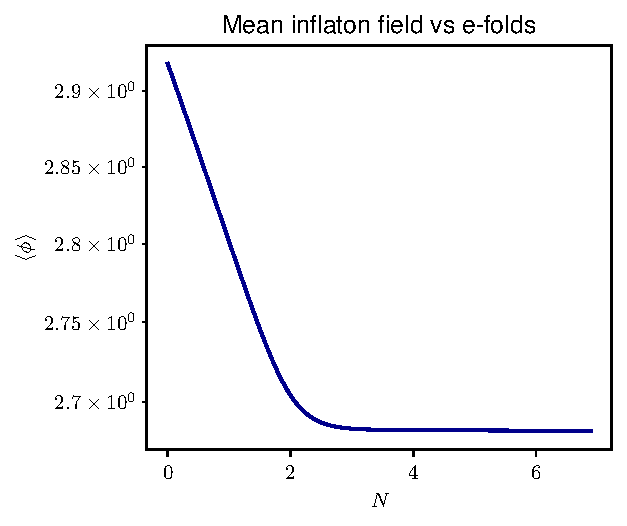
\includegraphics[width=0.483\linewidth]{phi.pdf}
    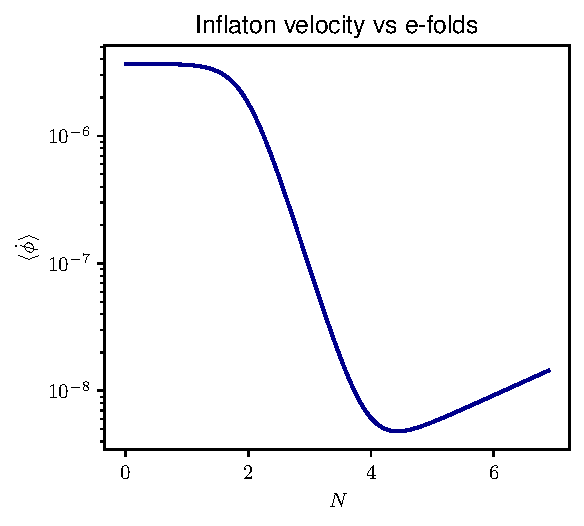
\includegraphics[width=0.45\linewidth]{phidot.pdf}
    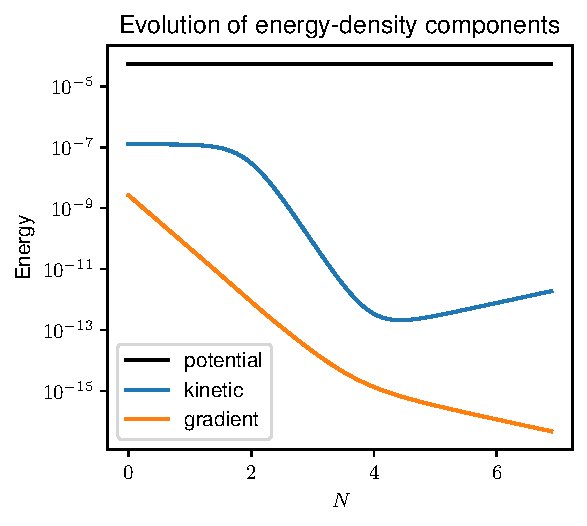
\includegraphics[width=0.45\linewidth]{energy.pdf}
    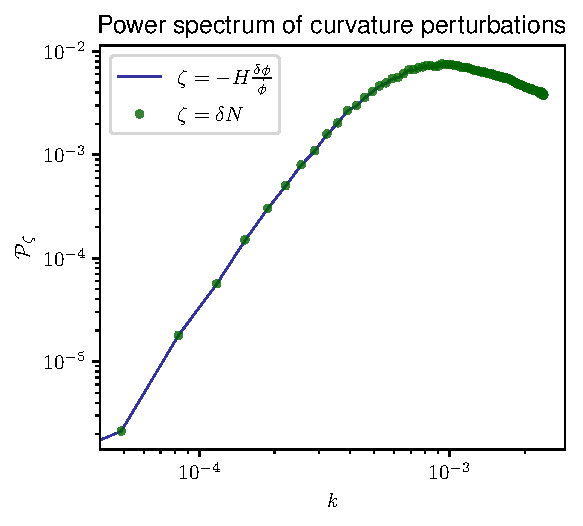
\includegraphics[width=0.45\linewidth]{spectrum.pdf}
 
    

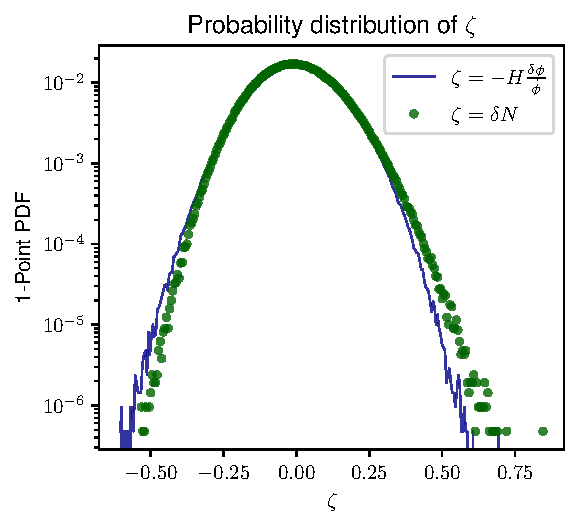
\includegraphics[width=0.46\linewidth]{PDF.pdf}
    \space \space \space\space\space \space \space \space \space\space\space \space  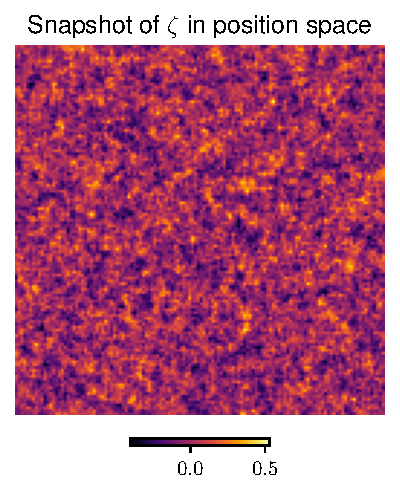
\includegraphics[width=0.34\linewidth]{snapshot.pdf}
    
    \caption{Example of typical outputs from the lattice simulation. \textbf{Top:} Evolution of the spatial average of the inflaton field and its velocity as a function of the number of $e$-folds $N$. \textbf{Middle:} Left panel shows the evolution of the different energy components in the lattice; right panel displays the power spectrum of the curvature perturbation $\zeta$, computed both via the linear relation and the fully nonlinear $\delta N$ formalism. \textbf{Bottom:} Left panel shows the probability distribution function (PDF) of $\zeta$; right panel shows a 2D slice of the final $\zeta$ field in position space. These outputs correspond to the default example in the code—namely, the ultra-slow-roll (USR) potential producing a peak in the power spectrum—run on a lattice with $N^3_{\rm pts} = 128^3$ points. These plots are generated using the example notebook \texttt{plot.ipynb}, included in the public release under the \texttt{notebooks/} directory.
  }
    \label{fig}
\end{figure}

\subsection{Default Options}
\label{sec:default}

The code includes two default potential options:

\begin{itemize}
    \item \textbf{Ultra-slow-roll potential}: A numerical potential featuring an inflection point that generates a pronounced peak in the primordial power spectrum. This corresponds to one of the Case I potentials in \cite{Caravano:2024moy, USR2}, specifically the one with a tree-level peak amplitude of the power spectrum\footnote{In \cite{Caravano:2024moy,USR2}, we classify the potentials using the tree-level power spectrum, i.e., the one predicted by linear perturbation theory.} of $\mathcal{P}_{\zeta,\rm tree}^{\rm peak} \sim 10^{-2}$. This potential does not have an analytic form and is instead loaded from files in the \texttt{inputs/} directory.

    \item \textbf{Quadratic potential}: An analytic potential given by \begin{equation}
    V(\phi) = \frac{1}{2}m^2\phi^2.
    \end{equation}
\end{itemize}
To toggle between the two options, change the following line in \texttt{parameters.h}:

\begin{lstlisting}[language=C++, firstnumber=3,caption={}]
// Set to 1 to enable a numerical potential loaded from file, 0 for analytic expression
#define numerical_potential 1
\end{lstlisting}
By default, the code runs with the numerical USR potential on a lattice of size $N_{\rm pts}^3 = 128^3$, and runs until the scale factor reaches $a=1000$ (where $a=1$ at the start of the simulation), corresponding to approximately $N = \log(1000) \simeq 6.9$ e-folds of evolution. The total number of e-folds should be chosen depending on the lattice resolution. See the next section for how to set the total number of e-folds for a given lattice size.

Running this benchmark code, including the $\delta N$ calculation to compute $\zeta$ from the lattice, on a machine with an Intel(R) Core(TM) i5-1038NG7 CPU @ 2.00\,GHz and 16\,GB RAM, compiled with \texttt{Apple clang 16.0.0}, takes 18 minutes and 31 seconds. Without the $\delta N$ calculation, it takes 10 minutes and 27 seconds. This timing refers to the unparallelized version of the code. If OpenMP is available on your system, you can expect improved performance depending on the number of cores.


\subsection{Configuring a New Potential}
\label{sec:configuring}

To use a different potential, follow these two steps:

\subsubsection*{Step 1: Define the Potential}

For an analytic potential, edit the following functions in \texttt{potential.cpp}:

\begin{lstlisting}[language=C++, firstnumber=14,caption={}]
float analytic_potential(float field_value) {
    return 0.5 * m2 * pw2(field_value) / pw2(rescale_B);
}

float analytic_potential_derivative(float field_value) {
    return field_value * m2 / pw2(rescale_B);
}
\end{lstlisting}
These return the potential and its derivative. Modify them as needed for your model.

For a numerical potential, update the files in \texttt{inputs/}: 
\begin{itemize}
    \item \texttt{field\_values.dat}: field points $\phi$ at which $V(\phi)$ is evaluated
    \item \texttt{potential.dat}: values of $V(\phi)$
    \item \texttt{potential\_derivative.dat}: values of $V'(\phi)$
\end{itemize}
All files must be single-column. Note that running simulations with an analytic potential is much faster than interpolating a numerical potential.

\subsubsection*{Step 2: Set Parameters in \texttt{parameters.h}}

Once the potential is defined, the next step is to configure the relevant parameters in the \texttt{parameters.h} file. This file includes brief explanations of each parameter, but here we provide a more detailed guide to setting them appropriately.

The first parameters to set are the physical parameters of the potential. For example, for the quadratic potential, one of the default models, this reads:
\begin{lstlisting}[language=C++, firstnumber=55,caption={}]
const float m2 = 0.263e-10; // Mass squared for quadratic potential
\end{lstlisting}
This defines the inflaton mass squared, which determines the overall amplitude of the potential. If your model includes more than one parameter (e.g. a coupling or a second mass scale), you should declare each of them in this section.

Next, set the field rescaling factor, referred to as $B$ in \cref{eq:rescaling}:
\begin{lstlisting}[language=C++, firstnumber=56,caption={}]
const float rescale_B = sqrt(V0); // Field rescaling factor
\end{lstlisting}
This parameter sets the code units for both the time derivatives and the lattice spacing. A typical and convenient choice is to use either the value of the Hubble rate or the inflaton mass at the beginning of the simulation. All dimensionful quantities in the simulation are rescaled by this factor, so this choice determines the unit system in which the simulation runs.

After the physical parameters and code units are defined, you must set the initial value of the homogeneous field and its first time derivative in code units:
\begin{lstlisting}[language=C++, firstnumber=57,caption={}]
const float initial_field = 14.5; // Initial field value
const float initiale_derivative = -0.81529; // Initial field velocity (in code units)
\end{lstlisting}
These values set the starting point for the background evolution. In the case of the quadratic potential, for instance, an initial value of $\phi=14.5$ corresponds to roughly 53 $e$-folds of inflation remaining, meaning the simulation probes scales relevant for the CMB. 

You must also choose the comoving box size of the lattice:
\begin{lstlisting}[language=C++, firstnumber=57,caption={}]
const float L = 2.; // Comoving box size in code units (must be sub-horizon at start) 
\end{lstlisting}
The comoving size $L$, together with the number of lattice points $N_{\rm pts}$ (also set in \texttt{parameters.h}), determines the infrared and ultraviolet cutoffs of the simulation \cite{Caravano:2021pgc}:
\begin{equation}
k_{\rm IR} = \frac{2\pi}{L},\quad\quad k_{\rm UV} = \frac{2\sqrt{3}}{L}N_{\rm pts}.
\end{equation}
To ensure accurate initial conditions, the comoving box size must be smaller than the Hubble radius at the start of the simulation, i.e., $L \lesssim 1/(aH)$. A common choice is $L \sim 1/(aH)$, which guarantees that most modes begin well inside the horizon, avoiding unnecessarily long simulations. Note that in this case, the lowest-$k$ mode ($k_{\rm IR}$) may not be accurately initialized. However, the rest of the spectrum is well resolved, and this typically has negligible impact on the overall evolution.

The value of $N_{\rm pts}$, which sets the lattice resolution and UV cutoff, must be balanced against computational cost. Larger values of $N_{\rm pts}$ yield higher resolution, but increase the memory and runtime requirements. For example, simulations larger than $N^3_{\rm pts} = 128^3$ may be difficult to run on a laptop.

The final simulation time is set by specifying the final value of the scale factor:
\begin{lstlisting}[language=C++, firstnumber=25,caption={}]
// Final scale factor value (simulation stops when a >= af)
const float af = 1000.;
\end{lstlisting}
This value should be large enough to ensure that the comoving box is well outside the horizon by the end of the simulation. Extending the simulation significantly beyond the time when the box becomes super-horizon is typically unnecessary and does not affect the dynamics: at that point, no new modes enter the horizon due to the finite UV resolution of the lattice. This remains true unless the chosen potential exhibits interesting super-horizon dynamics, in which case it may be worth running the simulation for a longer time.

As part of a convergence test, it is recommended to vary the values of $L$ and $N_{\rm pts}$ to verify that the physical results do not depend on the lattice cutoffs. This is a standard consistency check in lattice simulations. Note, however, that in some models (particularly those with strong scale dependence), physical quantities may naturally depend on the cutoffs. In those cases, the goal is not to eliminate cutoff dependence but to determine whether it is a physical feature or a numerical artifact.

Another crucial parameter is the time step for the numerical integration:

\begin{lstlisting}[language=C++, firstnumber=60,caption={}]
const float dt = 0.00005; // Time step
\end{lstlisting}

The time step must be small enough to ensure stability and accuracy. A good practice is to rerun the simulation with different values of \texttt{dt} and check that the results remain unchanged. These convergence tests can be performed, at first, on small grids (e.g., $64^3$) to save time in determining a reasonable range of $dt$ values.

The time step and final time for the $\delta N$ calculation are specified separately:
\begin{lstlisting}[language=C++, firstnumber=66,caption={}]
const float dN = 0.0000001; // e-fold increment in deltaN evolution
const float Nend = 0.001; // Final e-folding time for deltaN run
\end{lstlisting}
Choosing these parameters requires some care. The step size \texttt{dN} must be small enough to resolve the evolution of the separate-universe equation (\cref{eq:eom_deltaN}). As a rule of thumb, it should be much smaller than the expected amplitude of the curvature perturbation, i.e. $\delta N \ll \sqrt{\mathcal{P}_{\zeta}}$. For very small $\mathcal{P}_{\zeta}$, the required step size becomes prohibitively small, and the $\delta N$ calculation is typically unnecessary—nonlinear effects are only important for $\mathcal{P}_{\zeta} \gtrsim 10^{-3}$, as shown in~\cite{USR2}.

The final time \texttt{Nend} should be long enough for all lattice points to reach a common final constant-field hypersurface $\phi_{\rm ref}$. By default, the simulation sets this surface automatically to the field value that minimizes the energy density at the end of the run. However, this choice may be problematic in models with multiple minima or extended plateaus. In such cases, the user can manually define the hypersurface by uncommenting the following line:
\begin{lstlisting}[language=C++, firstnumber=68,caption={}]
// const float phiref_manual = value; // (Optional) manually set the reference $\phi$ value
\end{lstlisting}
When this line is uncommented and a value is provided, the $\delta N$ calculation will use the manually specified reference field value instead of determining it dynamically.


\section{Conclusions and Outlook}
\label{sec:conclusions}

\texttt{InflationEasy} provides a lightweight and accessible framework to simulate single-field inflation on a three-dimensional lattice. Unlike previous lattice codes, which were primarily developed for preheating or post-inflationary dynamics, \texttt{InflationEasy} is tailored specifically to the inflationary phase itself. This includes features such as proper initialization of Bunch-Davies fluctuations using the lattice-corrected dispersion relation, as well as the direct computation of the comoving curvature perturbation $\zeta$ via a nonlinear $\delta N$ method.

While the code builds on well-established lattice field theory techniques and inherits structural elements from \texttt{LATTICEEASY}, it introduces several improvements designed specifically for inflationary studies, including an improved treatment of Fourier-space observables that takes into account the lattice dispersion relation. The code has been tested across a range of models, including models of inflation with enhanced small-scale fluctuations \cite{Caravano:2024moy,Caravano:2024tlp,USR2}.

A major strength of \texttt{InflationEasy} is its simplicity. Despite being written in C++, the code is modular and easy to read, making it accessible even to users with limited programming experience. Physical and numerical parameters are configured in a single file, \texttt{parameters.h}, while the inflationary potential can be modified by editing two functions in \texttt{potential.cpp}. Although the code includes basic OpenMP parallelization, it remains lightweight and can run efficiently on a wide range of machines, including personal laptops for moderate lattice sizes.

Looking ahead, future extensions of the code will include support for multifield models. We also plan to implement a gravitational wave module for computing tensor spectra sourced by field dynamics during inflation. Additional improvements, such as more efficient parallelization, higher-order spatial derivatives, are under consideration for future releases.

We hope \texttt{InflationEasy} will serve as a useful tool for both model builders and phenomenologists exploring the nonlinear dynamics of inflation, particularly in regimes where analytical methods are insufficient. We welcome feedback, contributions, and suggestions via the public repository at ~\textcolor{red}{[link]}.

	%%%%%%%%%%%%%%%%%%%%%%%%%%%%%%%%%%%
	\section*{Acknowledgements}
	%%%%%%%%%%%%%%%%%%%%%%%%%%%%%%%%%%%
	
	The author thanks Gabriele Franciolini, Drew Jamieson, Eiichiro Komatsu, Kaloian D. Lozanov, Mauro Pieroni, S\'ebastien Renaux-Petel, and Denis Werth for insightful discussions and comments. This work was supported by the Initiative Physique des Infinis (IPI), a research training program of the Idex SUPER at Sorbonne Universit\'e.
	
	\bibliographystyle{jhep}
	\bibliography{main}
	
\end{document}

